\documentclass[tikz,border=4pt]{standalone}
\usepackage{tikz}

\begin{document}
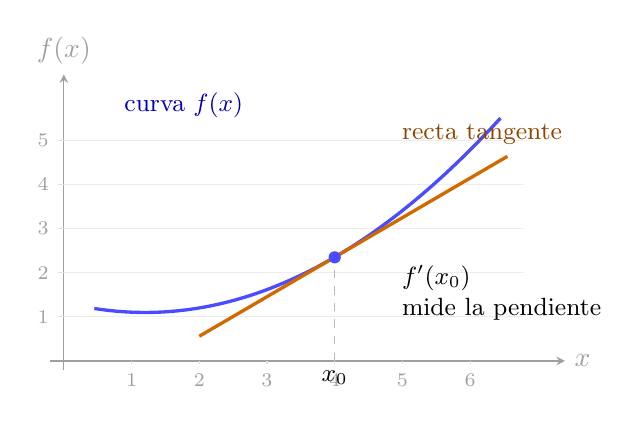
\begin{tikzpicture}[x=0.86cm,y=0.56cm,>=stealth]
  \draw[->,gray!75] (-0.2,0) -- (7.4,0) node[right] {$x$};
  \draw[->,gray!75] (0,-0.2) -- (0,6.5) node[above] {$f(x)$};

  \foreach \x in {1,2,3,4,5,6} {
    \draw[gray!25] (\x,0) -- (\x,-0.08) node[below,gray!75] {\scriptsize \x};
  }
  \foreach \y in {1,2,3,4,5} {
    \draw[gray!14] (0,\y) -- (6.8,\y);
    \draw[gray!25] (0,\y) -- (-0.08,\y) node[left,gray!75] {\scriptsize \y};
  }

  \draw[domain=0.45:6.45,samples=100,smooth,very thick,blue!70]
    plot ({\x},{0.16*(\x-1.2)*(\x-1.2)+1.1});

  \draw[very thick,orange!82!black] (2,0.56) -- (6.55,4.64);
  \draw[dashed,gray!55] (4,0) node[below,black] {\small $x_0$} -- (4,2.35);
  \fill[blue!70] (4,2.35) circle (2.2pt);

  \node[anchor=west,blue!70!black] at (0.75,5.8) {\small curva $f(x)$};
  \node[anchor=west,orange!55!black] at (4.85,5.15) {\small recta tangente};
  \node[anchor=west,align=left,black] at (4.85,1.55)
    {\small $f'(x_0)$\\[-1pt]\small mide la pendiente};
\end{tikzpicture}
\end{document}
